\chapter{Use Cases}

Use Case diagrams define tasks that users will perform to achieve a certain goal when using our incubating box and 3d bioprinter system.

\section{The Box}

\begin{figure}[H]
\caption{\label{figure:box-use-case} Use Case Diagram for The Box}
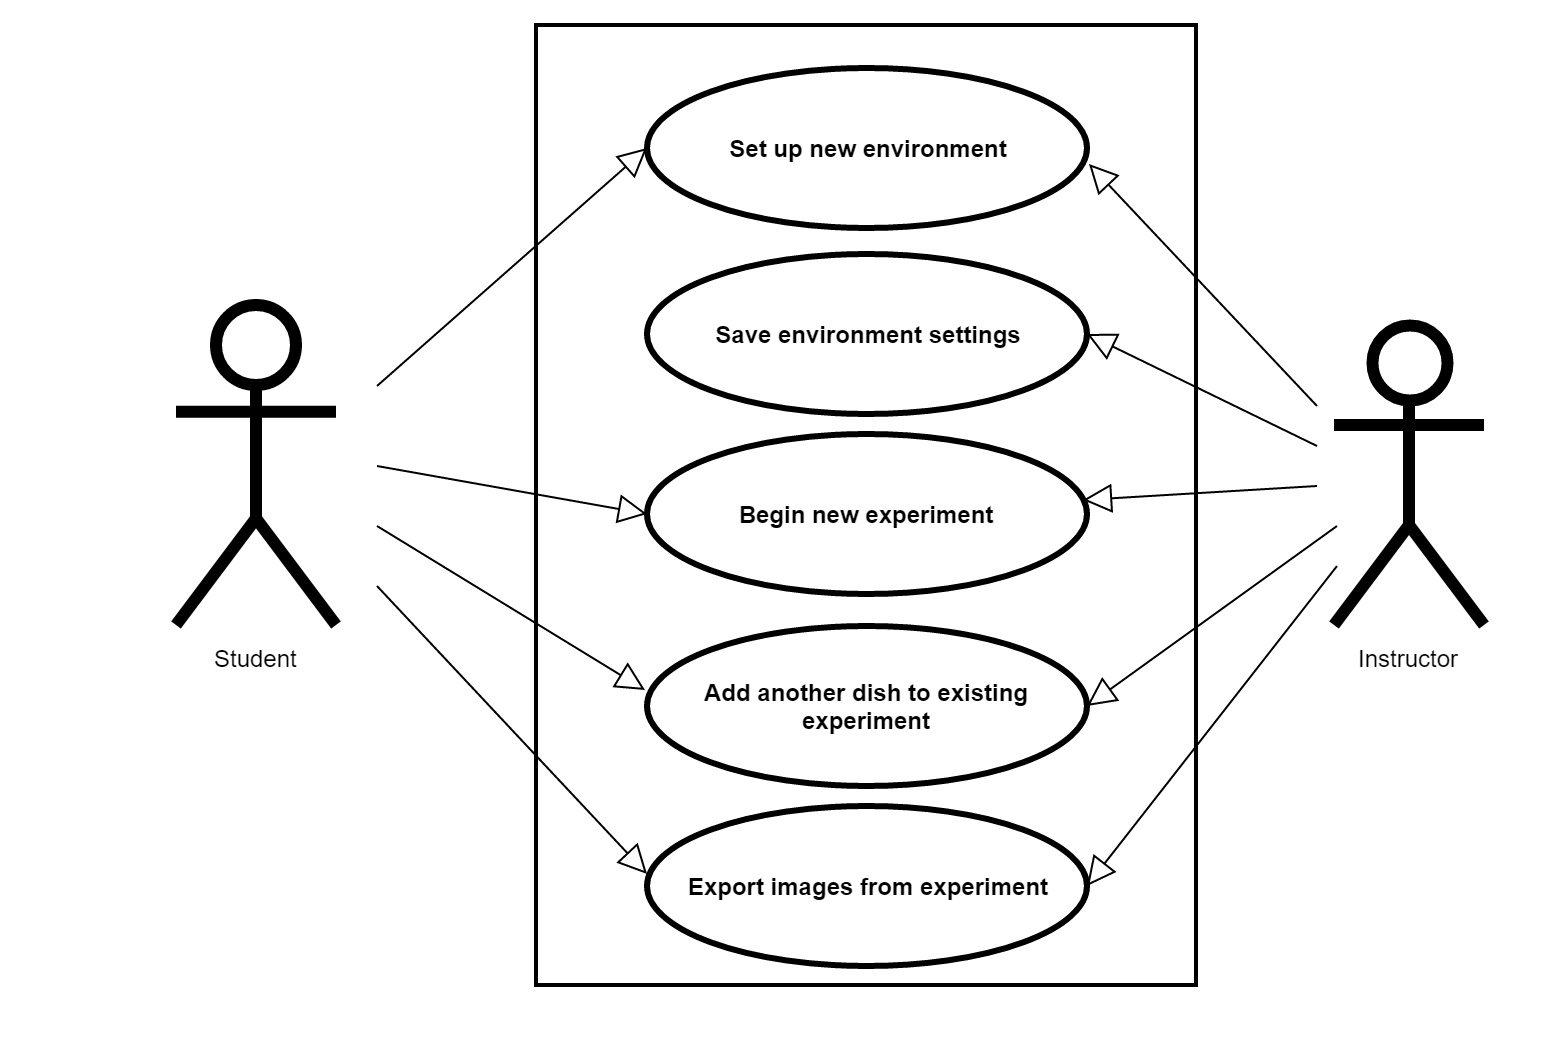
\includegraphics{box-use-case}
\end{figure}

\begin{enumerate}
	\item 
	\begin{itemize}
		\item Name: Set up new environment
		\item Goal: Prepare The Box to have the proper settings for the experiment that the user wants to run
		\item Actors: Student, Instructor
		\item Pre-conditions: No other experiment is currently running
		\item Steps: Either load settings that have been previously saved, or enter custom light, temperature, and image capture settings. 
		\item Post-conditions: The Box is at currect environment settings for the experiment.
		\item Exceptions
	\end{itemize}
	\item 
	\begin{itemize}
		\item Name: Save environment settings
		\item Goal: Save temperature, light, and image capture settings to prevent repetition in the future
		\item Actors: Student, Instructor
		\item Pre-conditions: User has input custom temperature, light, and image capture settings
		\item Steps: User clicks `Save Custom environment' and enters an appropriate name
		\item Post-conditions: Future users will now be able to load this environment for future experiments
		\item Exceptions: n/a
	\end{itemize}
	\item 
	\begin{itemize}
		\item Name: Begin new experiment
		\item Goal: Begin timer and image capture on current incubated experiment
		\item Actors:  Student, Instructor
		\item Pre-conditions: User has entered proper environment settings, selected which petri dishes are present, and has placed petri dishes in The Box. The Box has been brought to proper temperature.
		\item Steps: Click `Begin Experiment'
		\item Post-conditions: Timer and image capture begins
		\item Exceptions: n/a
	\end{itemize}
	\item 
	\begin{itemize}
		\item Name: Add another dish to existing experiment
		\item Goal: Add another dish to a experiment that is already running 
		\item Actors:  Student, Instructor
		\item Pre-conditions: An experiment must be running in The Box
		\item Steps: User places dish in the box. Clicks on the appropriate petri dish to begin timer and image capture of new dish
		\item Post-conditions: New petri dish is added into the experiment and final end time is extended to accommodate 
		\item Exceptions
	\end{itemize}
	\item 
	\begin{itemize}
		\item Name: Export images from experiment
		\item Goal: Download images captured during the experiment of a single petri dish for analysis
		\item Actors:  Student, Instructor
		\item Pre-conditions: A USB drive has been inserted and detected
		\item Steps: Click `download images' button, Select the relevant dish, click `download'
		\item Post-conditions: Images transferred onto the USB drive
		\item Exceptions
	\end{itemize}
\end{enumerate}
\section{Feasability Study}